\section{Dynamical Systems Formulation of Traffic Equilibrium}

The variational inequality formulation of the traffic equilibrium condition is a static condition.
Of particular interest in re-framing traffic equilibrium in the logic of differential hybrid games is to identify a dynamical system which not only preserves traffic equilibrium as an invariant but pushes a non-equilibrium state toward equilibrium.

\citet{nagurney1997projected} introduce a \textit{Projected Dynamical System} formulation of traffic equilibrium given by \eqref{eqn:project-dynamical-system}.

\begin{align}
    \mathbf{x}' &= \Pi_{\Omega}(\mathbf{x}, -\mathbf{t}(\mathbf{x}))\label{eqn:project-dynamical-system}\\
    \intertext{with link flow $\mathbf{x} \in \Omega$ and,}
    \Pi_{\Omega}(x, v) &= \lim_{\varepsilon\to 0}\frac{P_{\Omega}(x + \varepsilon v) - P_{\Omega}(x)}{\varepsilon}\\
        &= \lim_{\varepsilon\to 0}\frac{P_{\Omega}(x + \varepsilon v) - x}{\varepsilon}\\
    P_{K}(u) &= \arg\min_{v\in K} \| u-v\|
\end{align}

The operator $\Pi_{\Omega}$ can be thought of as a G\^{a}teaux directional derivative along the negative of the link cost of the norm projection onto $\Omega$, $P_{\Omega}$ for $x\in \Omega$.
Under this model, link flows change in the feasible direction that offers the largest reduction in the users travel costs.
It's important to note that solutions of \eqref{eqn:project-dynamical-system} are not functions of real time.
The main result presented in \citet{nagurney1997projected} is to show that one my discretize \eqref{eqn:project-dynamical-system} to produce an algorithm which converges on the true solution.
In this setting, we may think of this system as representing, somewhat counter-intuitively, the long term evolution of traffic flow.

As a thought experiment consider the morning commute.
This is an oft-used application of the static traffic assignment problem because in this setting the assumption that travel demand is constant is not so unbelievable: commuters tend to leave the same house at the same time headed toward the same place as they did the morning before.
On day $i$ the commuters choose their routes, $\mathbf{x}_{i}$, based on the link costs from the day before, $\mathbf{t}(\mathbf{x}_{i-1})$.
If they can perturb their route to achieve a lower travel time \textit{based on yesterday's link costs}, they do.
What results is exactly a route choice $\mathbf{x}_i = P_{\Omega}(\mathbf{x}_{i-1}-\varepsilon \mathbf{t}(\mathbf{x}_{i-1}))$ for some $\varepsilon \geq 0$.

We repeat three important theorems proved in \citet{nagurney1997projected}.

\begin{theorem}
    \label{thm:correspondence}
    A link flow $x^*\in \Omega$ satisfies the variational inequality problem \eqref{eqn:ui-vi} if and only if it is a stationary point for the differential equation \eqref{eqn:project-dynamical-system}, that is,
    $$0= \Pi_{\Omega}(\mathbf{x}, -\mathbf{t}(\mathbf{x}))$$
\end{theorem}

\begin{definition}[Stability]
    \label{def:stability}
    The route choice adjustment process given by \eqref{eqn:project-dynamical-system} is \textbf{stable} if for every initial flow pattern $\mathbf{x}_0\in \Omega$ and every equilibrium flow pattern $\mathbf{x}^*$, the distance $\|\mathbf{x}^* - \mathbf{x}_0(s)\|$ is monotone non-increasing in $s$.
\end{definition}

\begin{theorem}
    The route choice adjustment process is \textit{stable} if the link cost $t$ is monotone increasing in the link flow.
\end{theorem}

\begin{definition}[Asymptotic Stability]
     The route choice adjustment process given by \eqref{eqn:project-dynamical-system} is \textbf{asymptotically stable} if it is stable and, for any initial flow pattern $\mathbf{x}_0\in \Omega$ there exists some  equilibrium flow pattern $\mathbf{x}^*$ such that $\mathbf{x}_0(s) \to \mathbf{x}^*$ as $s\to \infty$.
\end{definition}

\begin{theorem}
    \label{thm:convergence}
    The route choice adjustment process is \textit{asymptotically stable} if the link cost $t$ is strictly monotone increasing in the link flow.
\end{theorem}

\begin{figure}[!ht]
    \centering
    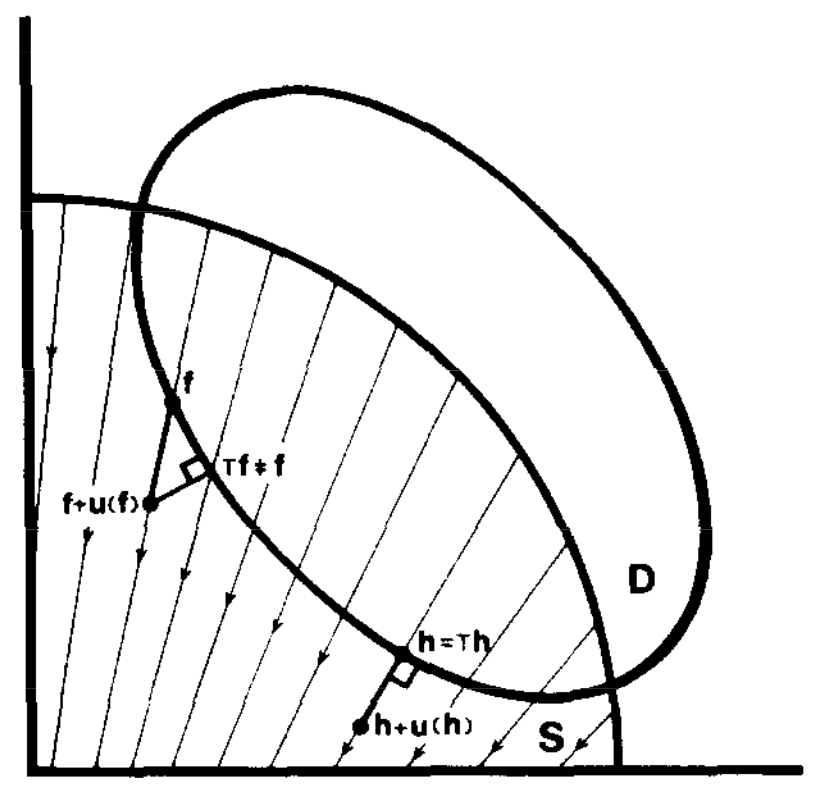
\includegraphics[width=0.4\textwidth]{figures/equilibrium-projection.png}
    \caption{Visual depiction of the dynamical system in \eqref{eqn:project-dynamical-system}. Here, $D\cap S$ represents the feasible region $\Omega$, $u(\cdot) = -t(\cdot)$ and $Tf$ is the projection of $f+u(f)$ onto $\Omega$. The vector field represents $u$. The flow $h$ is an equilibrium. We see that the equilibrium flow $h$ is a fixed point of $T$ whereas the $T$ applied to some non-equilibrium point $f$, is not a fixed point ($Tf \neq f$) and nudges the system toward equilibrium. The operator $\Pi_{\Omega}$ can be considered the infinitesimal version of the operator $T$ in the diagram.}
    \label{fig:equilibrium-projection}
\end{figure}

As a succinct visual aid of this process, consider \cref{fig:equilibrium-projection} re-printed here from  \citet{smith1979existence}. 
Lets consider how the route choice adjustment process acts on an arbitrary feasible link flow $x$ in \cref{fig:equilibrium-projection}.
Suppose $x$ is in the interior of $D\cap S$.
In this case, $x'$ is simply $-t$ and the link flow will evolve toward the boundary.
Upon reaching the boundary, $x$ can no longer move in the direction of $-t$ and remain in the feasible set.
The dynamics ensure this through use of the projection operator.
As a result, $x$ evolves in the direction most closely aligned with $-t$ that still points in the direction of $\Omega$.
The link flow will then move along the boundary, approaching the equilibrium point $h$.  
At the equilibrium point we see that $\Pi_{\omega}(h, -t(h))=0$ since $P_{\Omega}(h- \varepsilon t(h)) = h$ for all $\varepsilon \geq 0$.

From \cref{thm:correspondence} we see that $P \equiv \forall \mathbf{\tilde{x}} \in \Omega (\mathbf{t}(\mathbf{x})(\mathbf{\tilde{x}}- \mathbf{x}) \geq 0)$ is an invariant of the route choice adjustment process \eqref{eqn:project-dynamical-system}.
Moreover, \cref{thm:convergence} guarantees that following the route adjustment process will get us closer to equilibrium, or at least never lead us further from equilibrium.
Concretely, these two facts can be expressed in differential dynamic logic as follows.

\begin{theorem}
    The following is a valid formula.
    $$\forall \mathbf{\tilde{x}} \in \Omega (\mathbf{t}(\mathbf{x})(\mathbf{\tilde{x}}- \mathbf{x}) \geq 0) \implies [\mathbf{x}'=\Pi_{\Omega}(\mathbf{x}, -\mathbf{t}(\mathbf{x}))\ \&\ \mathbf{x}\in \Omega] \forall \mathbf{\tilde{x}} \in \Omega (\mathbf{t}(\mathbf{x})(\mathbf{\tilde{x}}- \mathbf{x}) \geq 0)$$
\end{theorem}

\begin{proof}
    By \eqref{eqn:ui-vi}, the pre-condition implies that $\mathbf{x}$ is an equilibrium point.
    By \cref{thm:correspondence}, we have that since $\mathbf{x}$ is an equilibrium point,  $\Pi_{\Omega}(\mathbf{x}, -\mathbf{t}(\mathbf{x})) = 0$.
    Therefore, $\mathbf{x}'=0$ and $\mathbf{x}$ will remain unchanged so the post-condition is true.
\end{proof}

\begin{theorem}
    Let $\Omega^*$ denote the set of equilibria.
    If $\mathbf{t}: \Omega_s \to \mathbb{R}^m_+$ is strictly monotone increasing then the following is a valid formula.
    $$\epsilon > 0\land \mathbf{x} \in \Omega \implies \langle \mathbf{x}'=\Pi_{\Omega}(\mathbf{x}, -\mathbf{t}(\mathbf{x}))\ \&\ \mathbf{x}\in \Omega\rangle (\exists \mathbf{x}^*\in \Omega^*\ \|\mathbf{x} - \mathbf{x}^*\| \leq \epsilon)$$
\end{theorem}

\begin{proof}
    Let $\mathbf{x}_0 \in \Omega$. Let $\mathbf{x}_0(s)$ denote the state of $\mathbf{x}_0$ after running the dynamics for duration $s\geq 0$.
    Note that by construction, the dynamics ensure that if $\mathbf{x}$ is in $\Omega$ initially then $\mathbf{x}$ will remain in $\Omega$ after running the dynamics for any duration, i.e. the domain constraint is always satisfied.
    By \cref{thm:convergence}, for every $\epsilon > 0$ there exists real number $N$ such that if $s > N$ then $\|\mathbf{x}_0(s) - \mathbf{x}\| \leq \epsilon$. 
    Concretely, we may take any $r > N$.
    Then $\mathbf{x}_0(r) \in \Omega$ and $\mathbf{x}_0(s) \in \Omega$ for all $0 \leq s \leq r$.
    Moreover, we have that there exists some $\mathbf{x}^*\in \Omega^*$  such that $\|\mathbf{x}_0(r) - \mathbf{x}^*\| \leq \epsilon$.
\end{proof}
